%%%%% Fichero de ejemplo LaTeX que ilustra el uso de la Hoja de Estilo %%%%%%
%%%%% Jornadas.cls para Jornadas Sarteco

\documentclass[twocolumn,twoside]{Jornadas}
\usepackage[utf8]{inputenc}
\usepackage[english]{babel}
\usepackage{listings}
\usepackage{algorithm}
\usepackage{algorithmicx}
\usepackage{algcompatible}
\usepackage{adjustbox}
\usepackage{graphicx}
\usepackage{color}
\usepackage{caption}
\captionsetup{font=footnotesize}
\usepackage[caption=false,font=footnotesize]{subfig}
%\setlength{\marginparwidth}{2cm}
%\usepackage{todonotes}
\usepackage{placeins}
\usepackage{hyperref}
\usepackage{url}
\usepackage{msc}
\usepackage{xcolor,colortbl}
\usepackage{hyperref}

\makeatletter
% \getcountref extracts the raw reference and
% results zero for undefined references.
% Caution: undefined references will not generate
% LaTeX warnings!
\newcommand*{\getcountref}[1]{%
	\expandafter\@getcountref\csname r@#1\endcsname
}
\newcommand*{\@getcountref}[1]{%
	\ifx#1\relax
	0% undefined reference
	\else
	\expandafter\@car#1\@empty\@nil
	\fi
}
\makeatother

\DeclareRobustCommand*{\citeinside}{\cite}

% -*- Ajustes LaTeX en relación a las figuras -*-
\setcounter{topnumber}{10}     % Max. numero de figs. on top
\setcounter{bottomnumber}{10}  % Max. numero de figs. abajo
\setcounter{totalnumber}{10}   % Max. numero de figs. por pagina
\renewcommand{\topfraction}{1} % Max. fraccion de pagina ocupada por figs.
\renewcommand{\bottomfraction}{1}
\renewcommand{\textfraction}{0}  % Min. fraccion de pagina ocupada por texto
\renewcommand{\floatpagefraction}{1} % Max. espacio de pagina solo con figs.

\definecolor{gray97}{gray}{.97}
\definecolor{gray75}{gray}{.75}
\definecolor{gray45}{gray}{.45}

\lstset{
     inputencoding=utf8,
     extendedchars=true,
     backgroundcolor=\color{gray97},
     %
     stringstyle=\ttfamily,
     showstringspaces = false,
     basicstyle=\scriptsize\ttfamily,
     commentstyle=\color{gray45},
     keywordstyle=\bfseries,
     linewidth=.98\columnwidth,
     xleftmargin=3mm,
     breaklines=true,
     numbers=left,
     numbersep=6pt,
     numberstyle=\tiny,
     numberfirstline = false,
     firstnumber=auto,
     breaklines=true,
     %
     escapeinside={(*@}{@*)},
     literate={á}{{\'a}}1 {é}{{\'e}}1 {í}{{\'i}}1 {ó}{{\'o}}1 {ú}{{\'u}}1 {ñ}{{\~n}}1
   }

\def\BibTeX{{\rm B\kern-.05em{\sc i\kern-.025em b}\kern-.08em
    T\kern-.1667em\lower.7ex\hbox{E}\kern-.125emX}}

\newtheorem{theorem}{Teorema}

\hyphenation{pa-ra-le-lis-mo pro-cee-dings}

%Directorios en los que se buscan las figuras
\graphicspath{{.}{./figures/}}
%%%%%%%%%%%%%%%%%%%%%%%%%%%%%%%%%%%%%%%%%%%%

\begin{document}

\title{
	Estimating time of a CAL module execution \\
	\large Statistic under AI and its application to engineering sciences
}

\author{%
     Jan Bielecki%
}

\maketitle
% Oculta las cabeceras y los números de página.
% Ambos elementos se añadirán durante la edición de las actas completas.
\markboth{}{}
\pagestyle{empty} 
\thispagestyle{empty} % Oculta el número de la primera página

\begin{abstract}
Abstract ...
\end{abstract}

\begin{keywords}
Machine learning, BalticLSC ...
\end{keywords}

%Añade los ficheros que necesites:

%!TEX root = main.tex
\section{Introduction}
\subsection{Context}

\begin{figure*}[!t]
	\centering
	\begin{minipage}{0.9\linewidth}
		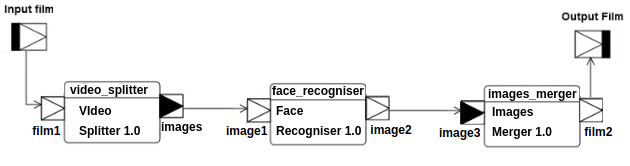
\includegraphics[width=1.0\textwidth]{face_recogniser_app}
	\end{minipage}
	\caption{\textit{Face Recogniser} scheme. Application written in the CAL language.}
	\label{fig:face_recogniser_app}
\end{figure*}

The research described in the article focuses on providing the tool for estimating the run-time of a single CAL module (data processing program or algorithm). Computation Application Language (CAL) is designed to write large-scale applications due to perform big data processing. Each CAL program consists of separately executed modules in sequence (with parallelization possibility) on virtual machines and sending the results further to the next module of the application. CAL language is a part of the system developed under the Baltic LSC\cite{baltic_lsc_website} project.

During the data processing within the application run, each module is executed with some input data. It could be a different kind of data e.g. data frame or set of images. The execution of a module is invoked on a virtual machine with limited resources (RAM, mCPUs, GPUs). The properties of input data and the execution environment resources will be used by models to estimate the overall application execution time and price on a specific cluster.

Baltic Large Scale Computing (BalticLSC\cite{baltic_lsc}) project is using CAL language to perform data processing tasks. Each task is an execution of a CAL application. CAL applications can use each module of the system in a reusable way. We can say that a single module is one block (commonly as a docker image) and an application is a schema of executing a sequence of blocks. Figure~\ref{fig:face_recogniser_app} shows the example application that consists of a few modules to perform face recognition on the input video data. Some sets of modules within a CAL application can be executed in parallel. Some modules can also be run as multiple instances of themselves to make data processing faster.

The demand for large-scale computation is tremendous and it is growing all the time. Mostly because of the high computational requirements of machine learning models and other tasks related to the Big Data thinks such as the Internet of Things~\cite{iot}. To execute the computations, it takes a lot of hardware resources. Moreover, it is really frequent that data processing programs have common parts that could be shared between them to make the whole process of the program's engineering more granulated and universal. Focused on just one-step of processing, an engineer could provide a well optimized module that could be shared in many programs. The BalticLSC project's research focuses on providing the complete system, handling mentioned challenges of large-scale computing.

\subsection{Issue}

The worst-case complexity of an algorithm is the greatest number of operations needed to solve the problem over input data of a given size. The analysis of algorithmic complexity emerged as a scientific subject during the 1960s and has been quickly established as one of the most active fields of study\cite{complexity}. The most common way to describe an algorithm complexity is the \textit{big O} notation (collectively called Bachmann–Landau notation or asymptotic notation) which is the universal formula that describes how the run-time of an algorithm grows as the input data size grows. 

In our work, we study the formula (more precise and complex one in comparison to the \textit{big O} notation) that takes mixed sets of input data and run-time environment properties as arguments. Moreover, the models we introduce in further parts will provide the estimation of the data processing program run-time and not only the complexity formula as the \textit{big O} notation does.

\subsection{Related work}

Since run-time estimation is a long-known issue, it is commonly studied from different perspectives and various approaches. There are many articles that, to some extent, coincides with the research carried out in this article. An overview of the problem with the list of possible, known solutions is described in the \textit{estimation of the execution time in real-time systems}\cite{wcet}. The authors focus on the \textit{WCET} concept. This project aims not to estimate execution time as a deadline that could not be exceeded. In our work, we try to estimate the average-case execution time (\textit{ACET}), which has a loser requirement for the final upper bound of the run-time than the \textit{WCET}.

A similar approach to the run-time estimation have been introduce in the \textit{Execution Time Analysis for Embedded Real-Time Systems}\cite{time-analysis} - as is said in the section 5. of the article, a static timing  analysis tool works by statically analysing the properties of the program (embedded to a specific structure like vector or graph) that affect its timing behavior. On the other hand, our approach is to statically analyze the properties of input data and the run-time environment resources. It allows to focus more on a single program and receive more accurate results. However, we have to provide a sufficient amount of input data for each module what is challenging. The fact that analysing programs run in BalticLSC system and they are reusable we assume that each module will be repeatedly triggered and it allows to carry enough data.  

In section 3.6 of the \textit{Using online worst-case execution time analysis and alternative tasks in real-time systems}\cite{images-processing-time} we can find a similar approach to carry out the regression using input data feature (section 3.6). The authors use an amount of image pixels as the only feature to estimate the execution time of a few different image processing algorithms. This is only a part of the whole approach for the worst-case execution time analysis described in the article, but it is the most related one to our work. It is worth noticing that there could be some specific input data properties for each algorithm that substantially impact the run-time. Models that we studied have general, strictly limited features, the same ones for each module, but one can extend it with some specific properties of a module.

To get a more precise run-time estimation results, one can study the program with similar input data. In the article \textit{A Prediction Model for Measurement-Based Timing Analysis}\cite{ga} the authors made an experiment by generating random lists of data with the same properties and then train the artificial neural network to predict the \textit{WCET}. They used \textit{Gem5} to simulate the run-time environment. We have used the docker as an execution environment which allows receiving more real data with a natural noise introduce to the response variable (execution time). The authors develop their work in the next article\cite{surogate} using the concept of surrogate models as a solution to the problem of generating training data. Such generating can increase overheads of the execution time estimation for processing algorithms with heavy input data. It is worth considering as an extension of our approach to generating some input data when the module is new and does not have any executions yet.

If we know that there will be not enough execution of each program within some system, we can create a single model for a whole system. The authors within the article \textit{Nonlinear approach for estimating WCET during programming phase}\cite{program-features} estimate a \textit{WCET} by extracting the program features from the object code. It starts when the source code of a program is successfully compiled into object code. Then, the extracted features were used for subsequent sample optimization and \textit{WCET} estimate. The authors use the SVR algorithm with RBF kelner as we did likewise. Having a set of features for each program, we can unify a model to a single instance and provide the features as a part of input data for the model. Another clue to the not enough amount of input data for a model is described in the article \textit{A solution to minimum sample size for regressions}\cite{small-n}. The authors explore the problem of a small amount of training data which also affects the result of our article. Testing data generation and simple algorithms for the run-time estimation are used to reduce the impact of a small n problem on the final results of our work.

\subsection{Contribution}

Despite the widely studied subject of estimating a program execution time, there is always a place to improve. Our work, presented in the article, contributes to the current knowledge of run-time estimation. We offer another perspective of solving the problem and one can find some valuable aspects of our work.

Most importantly, we used simple machine learning algorithms (\textit{SVR} and \textit{KNN}, more about the algorithms and how they fit the problem in the further sections) to estimate a program run-time. Creating a separate model for each module (program) instead of embedding the program structure to a vector of features or control flow graphs (CFGs) allows being more focused on each module separately. As input data features for our models, we determined the basic properties of a program’s input data together with the properties of the run-time environment of an execution. 



%!TEX root = main.tex
\section{Data}

To predict time of module execution we create a machine learning model for each module. With each execution of the module, within some application, we will get another data point to train our model. We will use the following features (explanatory variables)\footnote{As a docker container that will be used to execute a module do not use SWAP memory, RAM is not colerated with execution time. In this program we will not use modules with GPU support. Summarazing, the GPUs and RAM resources limits are not taken into account for modeling.} as an input data for the model:
\begin{enumerate}
	\item mCPU limit - called \textit{mili cores} - the fraction of a physical CPU used to carry out the module execution,
	\item total size of an input data,
	\item max element size of an input data (if the input data is a set of files type it is the biggest part of data to be processed),
	\item avg size of an input element,
	\item number of input data elements.
\end{enumerate}
This last three features makes sense only if the input data is a set of files. Otherwise, if the data is just a single file (e.g. data frame), the features set should be reduced to just the first two elements from the list above.

Obviously, our dependent value (that we are going to estimate) is an execution time of a module. The example data frame that will be used to train and validate our models is presented in the table~\ref{tab:example_df}.
\begin{table*}[!t]
	\centering
	\caption{\label{tab:example_df}The example data frame for models training and validations.}
	\begin{minipage}{0.9\linewidth}
	{\footnotesize
		\begin{tabular}{|c c c c c c >{\columncolor[gray]{0.9}}c|} 
			\hline
			Module ID & mCPU & total size [KB] & max size [KB] & average size [KB] & number of elements & time [ms] \\ [0.5ex] 
			\hline\hline
			1 & 1.1 & 12414 & 1341 & 871 & 21 & 7813 \\ 
			\hline
			1 & 0.5 & 12414 & 1341 & 871 & 21 & 12406  \\
			\hline
			1 & 3.6 & 54001 & 2190 & 891 & 82 & 9017 \\
			\hline
			... & ... & ... & ... & ... & ... & ... \\ [1ex] 
			\hline
		\end{tabular}
	}
	\end{minipage}
\end{table*}	

%!TEX root = main.tex
\section{Algorithms}
\subsection{Support Vector Regression}

As a one of machine learning algorithms to estimate time of a CAL module execution we will use \textit{Epsilon-Support Vector Regression}~\cite{svrc} (SVR) - it is based on Support Vector Machine (SVM, orginally named \textit{support-vector networks}\cite{svm}).

We will use SVR model with a RBF kernel\cite{rbf_kernel} which is the most known flexible kernel and it could project the features vectors into infinite dimensions. It uses Taylor expansion which is equivalent to use an infinite sum over the polynomial kernels. It allows to model any function that is a sum of unknown degree polynomials.

Using kernel, the resulting algorithm is formally similar, except that every dot product is replaced by a nonlinear kernel function. This allows the algorithm to fit the maximum-margin hyperplane in a transformed feature space. The RBF kernel have the following form:

\[ K_{RBF}(\vec{x}, \vec{x}') = \exp{(-\gamma||\vec{x} - \vec{x}'||)}\ \textnormal{, where:}\]
\begin{itemize}
	\item $ ||\vec{x} - \vec{x}'|| $ is the squared Euclidean distance between the two vectors of features,\newline
	\item $ \gamma $ - hyperparameter described in more details below.
\end{itemize}
In the SVR algorithm we are looking for a hyperplane \textit{y} in the following form:
\[ y = \vec{w} \vec{x} + b \textnormal{, where:}\]
\begin{itemize}
	\item $ \vec{x} $ - vector of features,
	\item $ \vec{w} $ - normal vector to the hyperplane \textit{y}, using a kernel the $ \vec{w} $ is also in the transformed space.
\end{itemize}
Training the original SVR means solving:
\[ \frac{1}{2}||w||^2  + C \sum_{i}^{N}(\xi_i+\xi_i^*) \textnormal{,}\]
with the following constraints:
\[ y_i - \vec{w}x_i - b \le \epsilon + \xi_i  \]
\[ -y_i + \vec{w}x_i + b \le \epsilon + \xi_i^*  \]
\[ \xi_i \xi_i^* \ge 0 \]
Figure~\ref{fig:svrc} shows the wanted hyperplane with marked \textit{$\xi$} and \textit{$\epsilon$} parameters.
As we already choosed the RBF kernel for the SVR algorithm, our modelling is simplified to just find the best values of the following hyperparameters\cite{svr}:
\begin{enumerate}
	\item \textit{C} -the weight of an error cost. The regularization\footnote{Regularization is a way to give a penalty to certain models (usually overly complex ones)} hyperparameer, have to be strictly positive. The example from the figure use l1 penalty (the library that we use to modelling use the squared epsilon-insensitive loss with l2 penalty). The strength of the regularization is inversely proportional to C. The larger value of C the more variance is introduced into the model. 
	\item \textit{epsilon} - It specifies the epsilon-tube within which no penalty is associated in the training loss function with points predicted within a distance epsilon from the actual value. As it is shown of the figure~\ref{fig:epsilon} the grey data points do not provide any penalty to the loss function because they are within the allowed epsilon range around the approximation\footnote{\label{figure_example}The figure is based on some example data and it only shows the hyperparameter influence on model.}.
	\item \textit{gamma} - The \textit{gamma} hyperparameter can be seen as the inverse of the radius of influence of samples selected by the model as support vectors. Increasing the value of \textit{gamma} hyperparameter causes the variance increase what is shown in the figure~\ref{fig:gamma}\footnotemark[\getcountref{figure_example}].
	
\end{enumerate}
\begin{figure}[!htb]
	\caption{Visualization of the SVR's epsilon parameter~\citeinside{epsilon}.}
	\centering
	\label{fig:epsilon}
	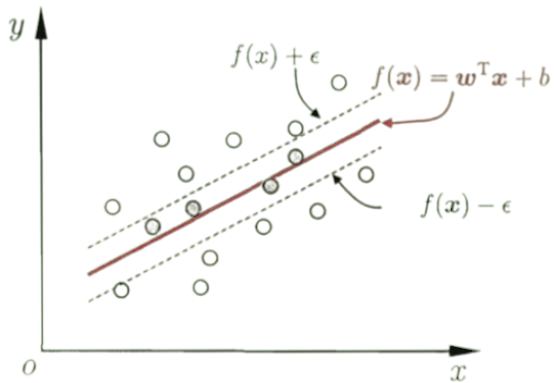
\includegraphics[width=0.45\textwidth]{epsilon}
\end{figure}
\begin{figure}[!htb]
	\caption{SVR's C parameter~\citeinside{svrc} influence on model.}
	\centering
	\label{fig:svrc}
	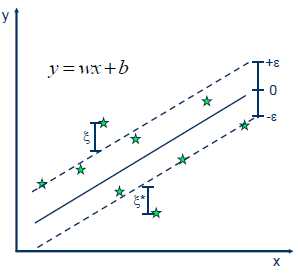
\includegraphics[width=0.45\textwidth]{svrC}
\end{figure}
\begin{figure}[!htb]
	\caption{SVR's gamma hyperparameter~\citeinside{gamma} influence on the model variance.}
	\centering
	\label{fig:gamma}
	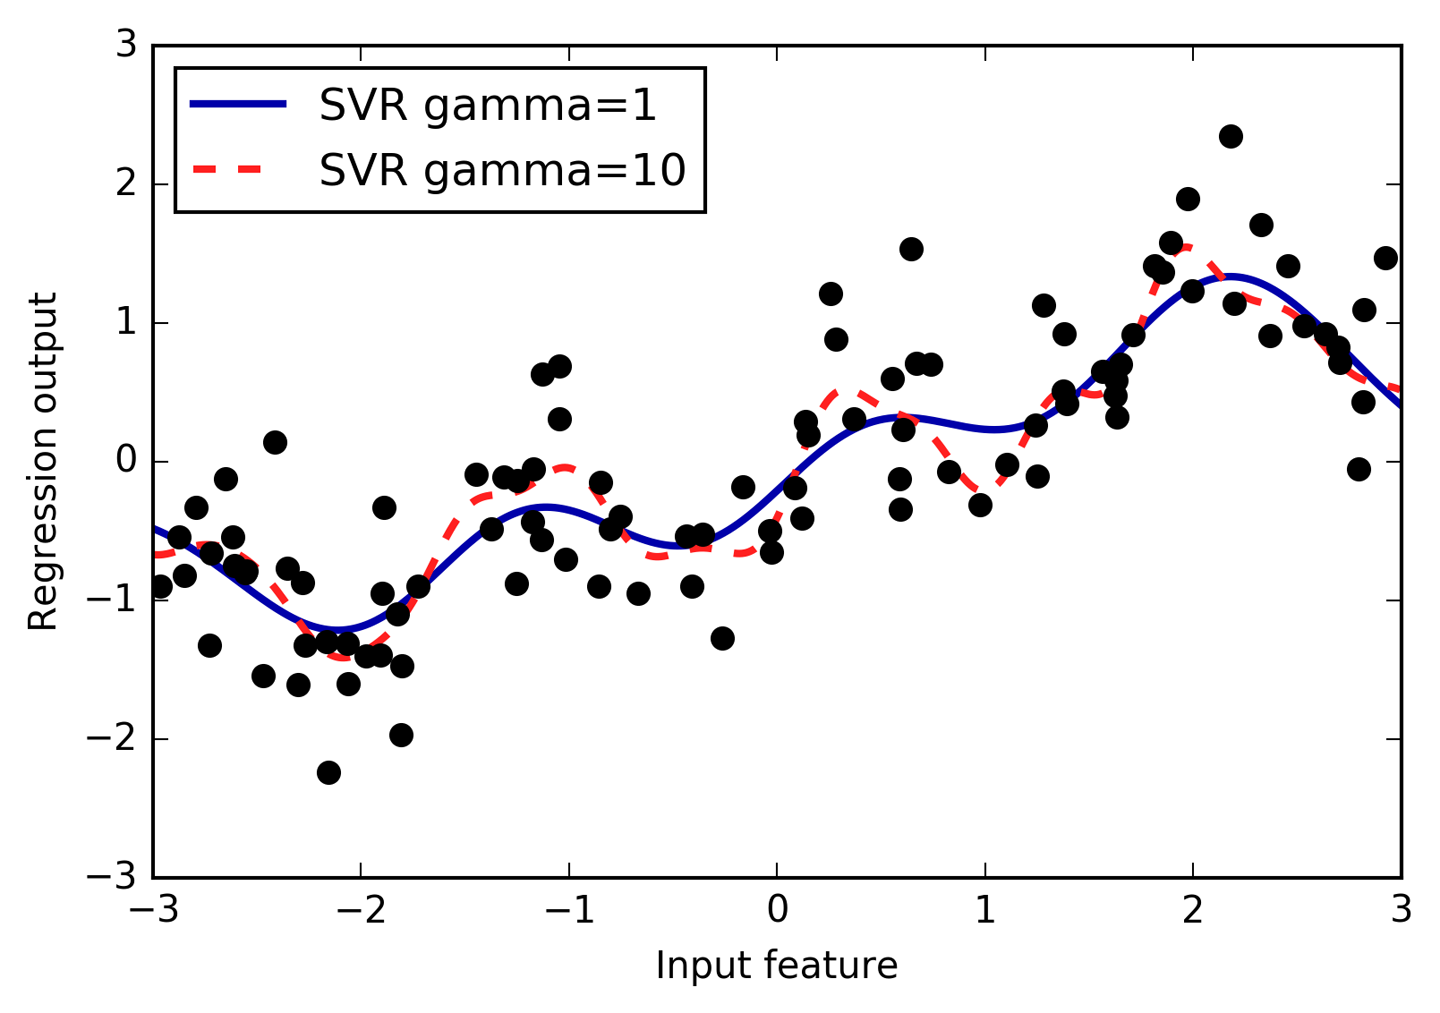
\includegraphics[width=0.45\textwidth]{gamma}
\end{figure}
You can find detailed information about C and gamma params in sklearn library documentation\cite{rbf_params}.

\subsection{K-nearest Neighbors Regression}

Another, examined algorithm used to estimating time of a module execution is a simple \textit{KNN}\footnote{\textit{KNN} - k-nearest neighbors} regression. Using the algorithm, a target is predicted by local interpolation of the targets associated of the nearest neighbors in the training set~\cite{knnreg}.In another words, the target assigned to a query point is computed based on the mean of the targets of its nearest neighbors.

To use the algorithm we have to define values of the following parameters:
\begin{enumerate}
	\item \textit{k} - number of the nearest neighbors
	\item \textit{weights} - weight function used in prediction. The basic nearest neighbors regression uses uniform weights: that is, each point in the local neighborhood contributes uniformly to the classification of a query point. Under some circumstances, it can be advantageous to weight points such that nearby points contribute more to the regression than faraway points. The weights can be calculated from the distances using any function for example the linear one.
	\item \textit{algorithm} - the procedure to calculate k-nearest neighbors for the query point. It does not have a direct impact to the final regression result, but the parameters of the algorithm surely have. For example, using the BallTree algorithm we have to choose the \textit{metric} parameter that will be used to calculate the distance between data points. It could be, for example, the Minkowski~\cite{minkowski} metric with the l2 (standard Euclidean~\cite{euclidean}) distance metric or any function that will calculate the distance between two points.
\end{enumerate}

\begin{figure}[!htb]
	\caption{KNN out of range fail.}
	\centering
	\label{fig:knn}
	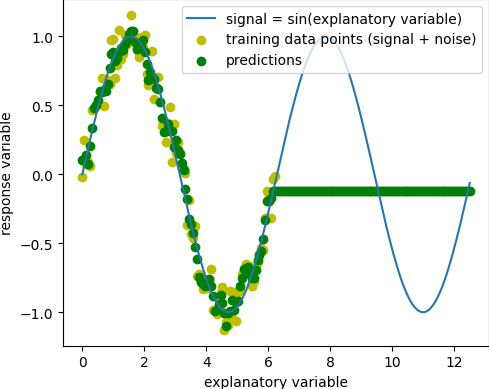
\includegraphics[width=0.5\textwidth]{knn}
\end{figure}
%!TEX root = main.tex
\section{Training and validation}
The training pipeline for each module contains the following steps:
\begin{enumerate}
	\item Having the 80 data points, we divide them into training and test data sets with 1:2 proportion.
	\item Standardization of a data set is a common requirement for many machine learning estimators: they might behave badly if the individual features do not more or less look like standard normally distributed data (e.g. Gaussian with 0 mean and unit variance)\cite{scaler}. We scale each column (feature) of the data set using the following formula:
	\[ \vec{x}_{f}^{'} = \frac{\vec{x}_{f}-\mu_f}{\sigma_f} \textnormal{, where:}\]
	\begin{itemize}
		\item $ \vec{x}_{f} $ - data set column \textit{f},
		\item $ \mu_f $ - mean of the column \textit{f},
		\item $ \sigma_f $ - standard deviation of the column \textit{f}.
	\end{itemize}
	\item Each algorithm have a few parameters that should be chosen wisely in order to the better results. It is hard to predict the best value of a continuous parameter. What we did is an exhaustive search over specified parameter values for an estimator from the given possible values. For each combination of the parameter values we validate the model using 5-fold cross validation on the training data set. It is called a \textit{grid search}\cite{grid_search}.
	\item Finally, we trained our model using the full training data set and the parameters that were found in the previous step.
	\subsection{Support Vector Regression}
	The parameters grid for the \textit{SVR} algorithm is listed below:
	\begin{lstlisting}[language=json,firstnumber=1]
'gamma': [0.0001, 0.0002, 0.0004, 0.0008, 
0.0016, 0.0032, 0.0064, 0.0128], 
'epsilon': [1e-06, 2e-06, 4e-06, 8e-06, 
1.6e-05, 3.2e-05, 6.4e-05, 0.000128, 
0.000256, 0.000512, 0.001024], 
'C': [1000.0, 2000.0, 4000.0, 8000.0,
16000.0, 32000.0, 64000.0, 128000.0, 
256000.0, 512000.0, 1024000.0, 2048000.0]
	\end{lstlisting}
	
	\subsection{K-nearest Neighbors}
	The parameters grid for the \textit{KNN} algorithm is listed below:
	\begin{lstlisting}[language=json,firstnumber=1]
'n_neighbors': [1, 2, 3, 4, 5, 6, 7, 8, 9, 10, 11], 
'weights': ['uniform', 'distance'], 
'p': [1, 2]
	\end{lstlisting}
	
	\subsection{Results}
	\begin{table*}[!t]
		\centering
		\caption{\label{tab:example_df}The results.}
		\begin{minipage}{0.9\linewidth}
			{\footnotesize
				\begin{tabular}{|c c c c >{\columncolor[gray]{0.9}}c|} 
					\hline
					Algorithm & Module name & best params & error [s] & relative error [\%] \\ [0.5ex] 
					\hline\hline
					\textit{SVR} & \textit{Video splitter} & 3131 & 3131 & 3.909 \\ 
					\hline
					\textit{SVR} & \textit{Face recogniser} & 1477 & 1477 & 1.981  \\
					\hline
					\textit{SVR} & \textit{XGB grid search} & 1229 & 1229 & 11.371 \\
					\hline
					\textit{SVR} & \textit{Images merger} & 1229 & 1229 & 11.371 \\ [1ex] 
					\hline
				\end{tabular}
			}
		\end{minipage}
	\end{table*}	
\end{enumerate} 


\subsection{Training}
...
\subsection{Validation}
...
%!TEX root = main.tex
\section{Conclusiones}

Conclusions ...
\url{https://github.com/rasenjop/Plantilla-Jornadas-Sarteco}.


\section*{Thanks}

Thanks for the help and support ...
%Comenta la línea \nocite para que sólo se incluyan en las referencias
%las entradas que esté referenciadas en el texto con \cite{}
\nocite{*}
\bibliographystyle{Jornadas}
\bibliography{biblio}

\end{document}
